\documentclass{article}
\usepackage{amsmath, amssymb, graphicx, subfigure, algorithmic, color,
booktabs}

\DeclareMathOperator*{\argmax}{arg\,max}

\author{Mitchell Koch, Justin Huang\\\{mhkoch,jstn\}@uw.edu}
\title{Learning Relation Entailment Graphs\\CSE 515 Final Report}
\date{Friday, June 14, 2013}

\begin{document}
\maketitle

\begin{abstract}

We study the problem of learning relation entailment graphs to represent relationships between predicates extracted from text, for the purpose of improving relation query performance. We use Bayesian network structure learning to learn a graph of relation entailments given results from a relation extraction system, and also leverage the WordNet resource, mapping relation strings to WordNet senses in order to use entailments in WordNet. Using these methods to expand relation queries, we find that Bayesian network structure learning reduces precision, because we were not able to find a way to bias the directionality of edges in a way appropriate for the problem. Using WordNet sense entailments with a logistic regression classifier to select which paths are likely, we increase the number of results returned by over 6x while increasing precision from 87.88\% to 91.43\% for 15 example queries from Open IE~\cite{Etzioni:2008:OIE:1409360.1409378}.
\end{abstract}

\section{Introduction and Motivation}

Relation extraction systems learn facts from natural language text of the form \textsf{relation(arg1, arg2)}, such as \textsf{capture(Caesar, Egypt)}. The relations can be within a fixed and finite schema, such as Freebase relations as in~\cite{HoffmannZLZW11} or they can be any strings in the text likely to represent a relation as in Open IE~\cite{Etzioni:2008:OIE:1409360.1409378}. Recently there has been work in learning both kinds of relations together using a matrix factorization approach~\cite{riedel13relation}.

The goal of relation entailment is to learn a directed graph between relations such that if a relation holds for certain arguments, its child relations should hold for the same arguments. Relation entailment should be helpful to improve relation extraction in any of the above contexts, in that results from relation extraction can be used to generate more results by following the relation entailment graph. This can also be helpful in serving the larger goal of question answering. Not every question can be answered directly from text, making inference using entailments important.

In this project, we focus on increasing the precision and yield of relation extraction results from Open IE using relation entailment and evaluate based on the database query task described below. Since relation entailment involves creating a directed graph over relations, a natural method to try is Bayesian network structure learning. We also use entailments over WordNet senses and learn what entailments are useful for relation entailment using logistic regression.

\subsection{Database Query Task}
\label{database-query-task}
We define the following database query task to evaluate a relation entailment graph. Let $R$ be a set of relation strings, and $A$ be a set of argument strings. We are given a database $D$ of facts, where each fact is of the form $r(x, y)$ for some $r\in R$ and $x, y\in A$.

Given a query for a relation $r$ with arguments $x$ and $y$, we can expand the query to additionally search for all $r^\prime(x, y)$ such that there exists an edge from $r^\prime$ to $r$ in the entailment graph. An example of this process is shown in figure~\ref{query-expansion}. We can then evaluate the correctness of the returned results.

\begin{figure}[h]
\begin{center}
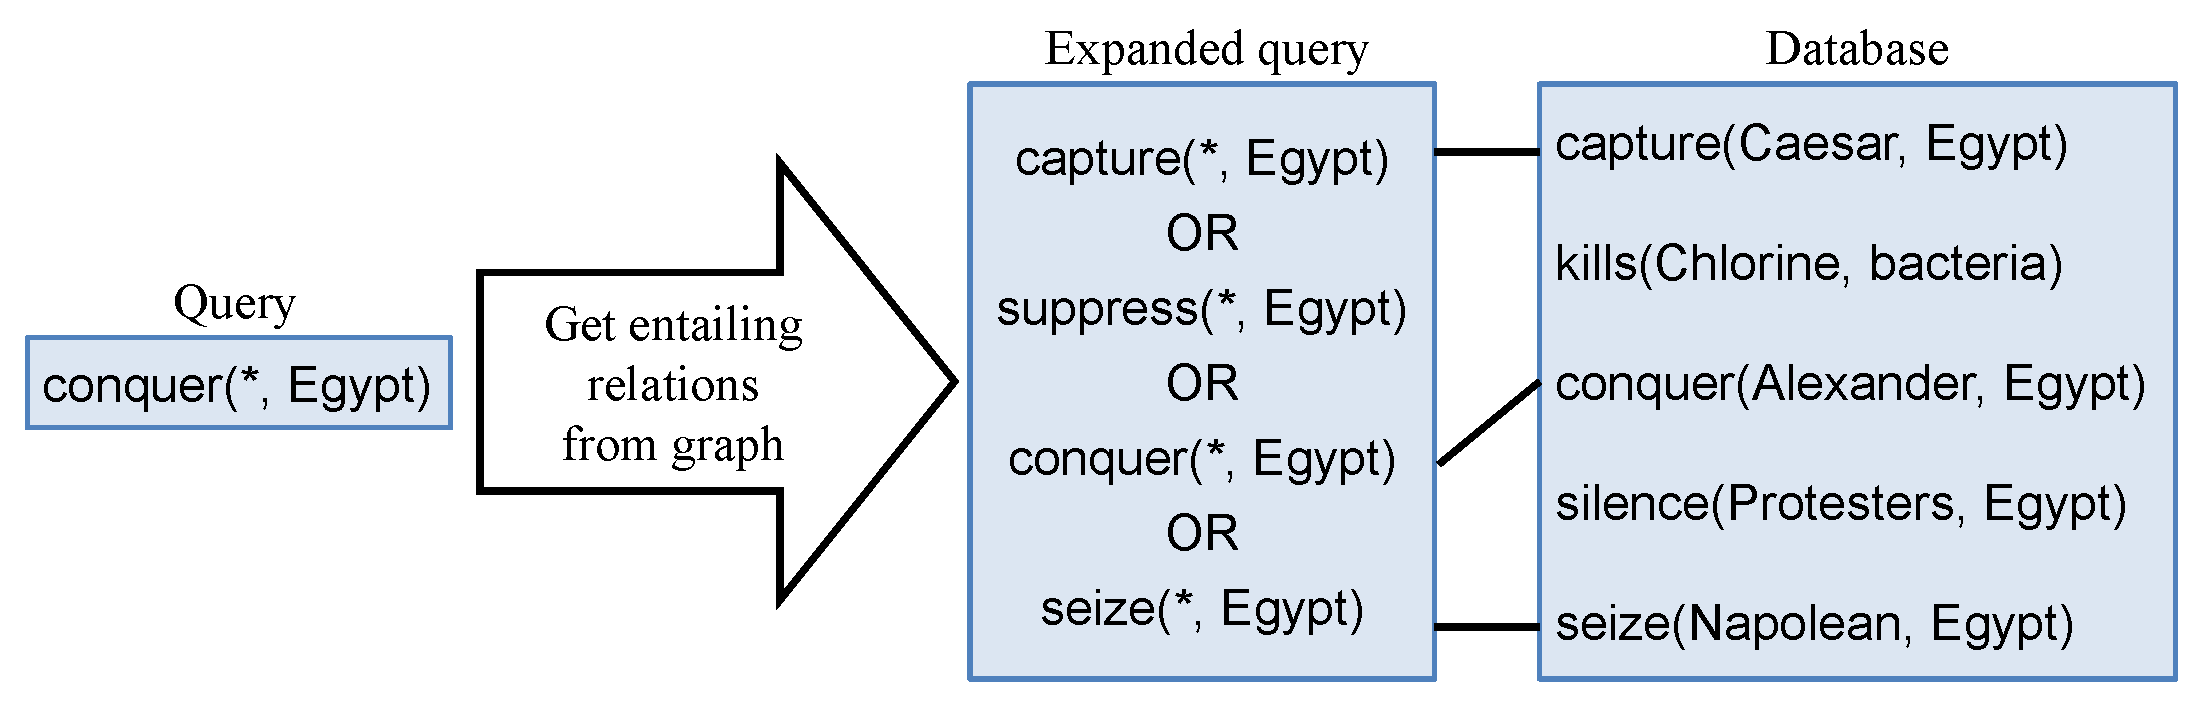
\includegraphics[width=1.0\textwidth]{figures/query-expansion.pdf}
\end{center}
\caption{An example of a query being expanded.}\label{query-expansion}
\end{figure}

\section{Methods and Algorithms}

\subsection{Constraints on WordNet}

WordNet~\cite{fellbaum98wordnet} is a hand-crafted resource that distinguishes between different word senses and provides synonyms and entailments between them. We denote a WordNet sense with a number where \textit{\#1} is the most common. For example \textit{note\#4} is the fourth most common sense of ``note,'' which means ``to write down''. Each WordNet sense has its sense number, a count indicating how often that sense is used, and a probability, which is the count divided by the sum of counts for all senses of the same word.

\subsubsection{WordNet Entailment Graph}
A troponym is a specialization of a word, e.g.\ ``to fly'' is a troponym of ``to travel.'' We say that WordNet sense $w_1$ entails $w_2$ if $w_1$ is a synonym of $w_2$, if $w_1$ is a troponym of $w_2$ in WordNet, or if there exists some $w_3$ such that $w_1$ entails $w_3$ and $w_3$ entails $w_2$. A path in the entailment graph is defined as the sequence of entailments between $w_1$ and $w_2$. The entailment graph is disconnected. Figure~\ref{wordnet-graph} shows one component of the graph, and figure~\ref{example-path} shows an example of a path in the graph, from \textit{note\#4} to \textit{write\#2}.

\begin{figure}[h]
\begin{center}
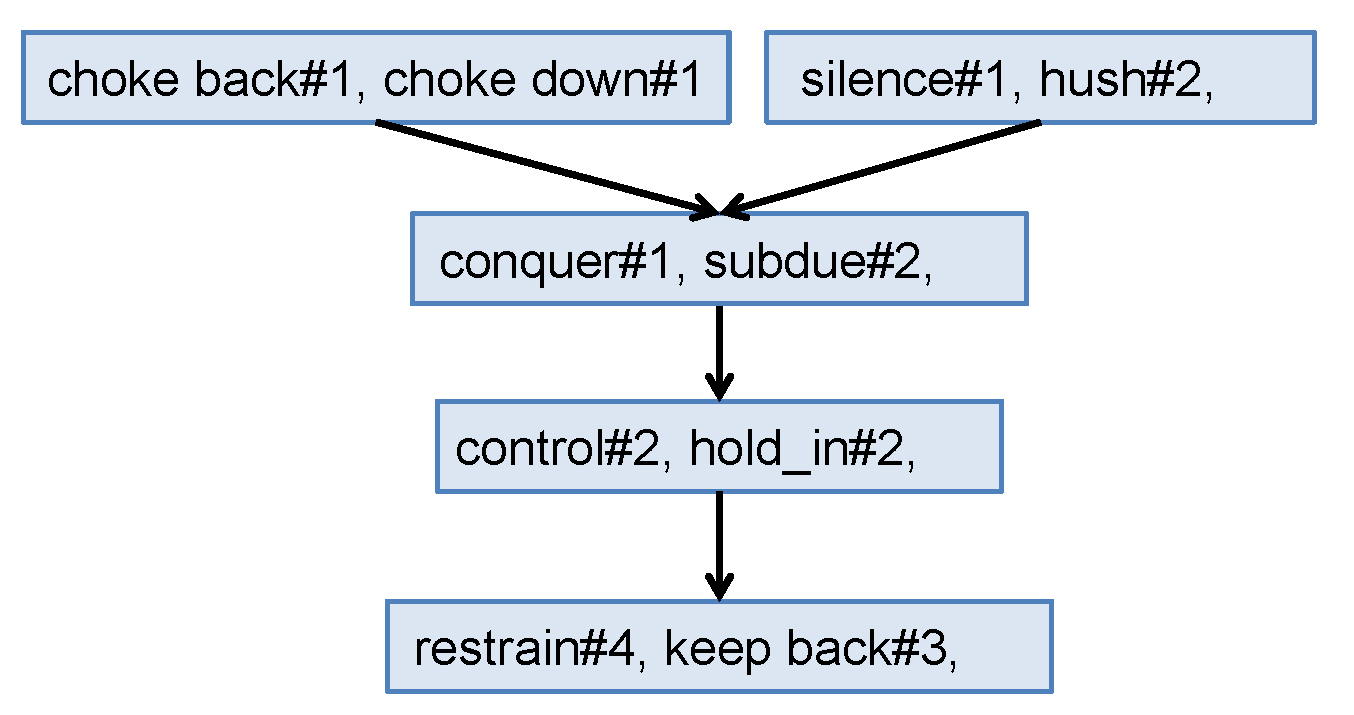
\includegraphics[width=0.6\textwidth]{figures/wordnet-graph.pdf}
\end{center}
\caption{Component of the WordNet entailment graph with the first sense of conquer, \textit{conquer\#1}. Boxes represent synonym sets, arrows represent entailments.}\label{wordnet-graph}
\end{figure}

\begin{figure}[h]
\begin{center}
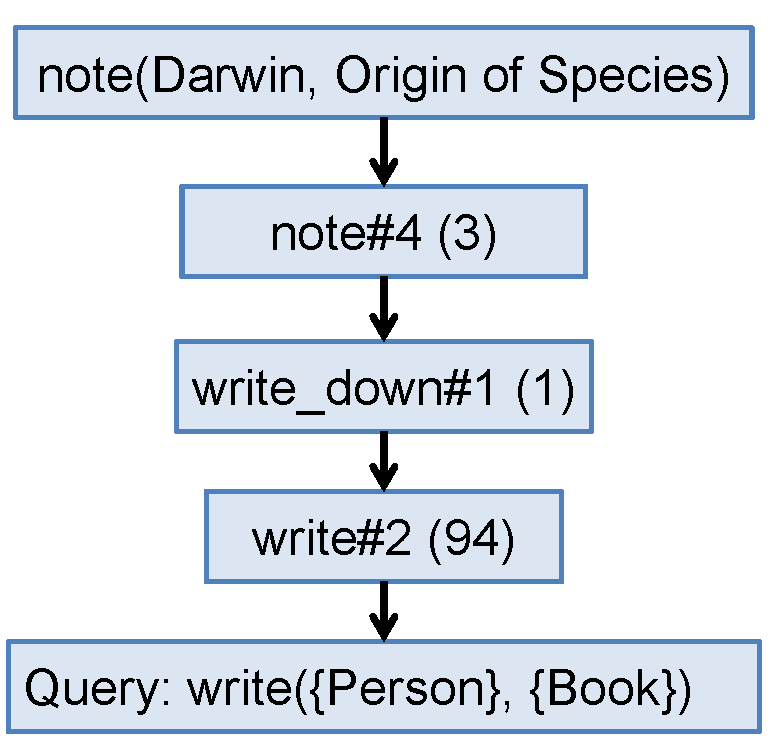
\includegraphics[width=0.4\textwidth]{figures/example-path.pdf}
\end{center}
\caption{Example path in entailment graph}\label{example-path}
\end{figure}

Although WordNet already defines an entailment graph between verb senses, one hurdle to using it is determining what sense to use. For example, given the verb ``take,'' is it \textit{take\#21} (take by force) or \textit{take\#2} (take time)? Each sense will lead to very different entailments. First we assume a string can take on any of its WordNet senses, which may lead to noisier entailments. Then we train a logistic regression classifier to help filter out noisy entailments.

\subsubsection{Logistic Regression Classifier}
For a certain set of queries, we use all possible entailments from WordNet on the database query task and label each fact as relevant to the query or not relevant to the query. This data is subsequently used to train the logistic regression model. For each result, we record the path that was taken in the entailment graph and produce the following features:
\begin{enumerate}
  \item Path length
  \item Average sense number
  \item Average WordNet probability
  \item Maximum sense number
  \item Minimum WordNet probability
\end{enumerate}

The length of the path is the number of nodes in the path. For example, in figure~\ref{example-path}, the length is 3. Because WordNet senses are ranked in order frequency, we use the average and maximum sense numbers as features, the idea being that an uncommon WordNet sense (e.g.\ \textit{take\#42}) could be a weak link in the entailment path. A similar intuition holds for the probabilities of the WordNet senses.

The output of logistic regression is a set of weights $w$ for each feature. Let $x$ be the vector of features described above. Then the probability of the label we would like to predict is given by:
\begin{align}
  P(x) = \frac{e^{w\cdot x}}{1 + e^{w\cdot x}}
\end{align} 

\subsection{Bayesian Network Structure Learning}

The problem of learning a network from data can be formulated as an
optimization problem: Given data ${\cal D}$, we want to find a Bayesian network ${\cal B}^{*}=({\cal G}^{*},\Theta^{*})$ to maximize
the posterior probability of the Bayesian network given the data:
\begin{eqnarray}
{\cal B}^{*}  =  \argmax_{{\cal B}}P({\cal B}|{\cal D}) & = & \argmax_{{\cal B}} P({\cal D}|{\cal B})P({\cal B}),\\
& = & \argmax_{{\cal G},\Theta} P({\cal D}|{\cal G},\Theta)P({\cal G},\Theta),\\
& = & \argmax_{{\cal G},\Theta} P({\cal D}|{\cal G},\Theta)P({\cal G})P(\Theta|{\cal G}).
\end{eqnarray}

The posterior probability of the graph prior assuming indendence of parameter priors, global parameter independence \cite{Friedman:full}, and parameter modularity \cite{Heckerman1995} yields

\begin{eqnarray}
P({\cal G}|{\cal D}) = P({\cal G})\prod_{i=1}^{n}\prod_{j=1}^{q_i}
\frac{\Gamma(N'_{ij})}{\Gamma(N'_{ij} + N_{ij})}
\prod_{k=1}^{r_i}\frac{\Gamma(N'_{ijk}+N_{ijk})}{\Gamma(N'_{ijk})} ,\label{eqn:dpsm}
\end{eqnarray}
where $q_i$ is the number of values for the parents of node $i$, $r_i$ is the number of values for node $i$, $N'_{ijk}$ is the Dirichlet distribution order for variable $i$
with value $k$ and parent value $j$, and $N'_{ij} =
\sum_{k=1}^{r_i}{N'_{ijk}}$. $N_{ijk}$ is the number of instances in ${\cal D}$ where $i$ with value $k$ has parents with value $j$ and  $N_{ij} =
\sum_{k=1}^{r_i}{N_{ijk}}$. This is derived in~\cite{Cooper1} and \cite{Chang}. In \cite{Chang}, this score metric is called the General Dirichlet Prior Score Metric (DPSM).

The number of model structures is super-exponential in the number of variables, making exact optimization intractable in general. Approximate approaches include direct search using hill climbing as well as Markov Chain Monte Carlo (MCMC) techniques as in~\cite{FK03}. For smaller graphs, with less than 20 nodes, dynamic programming techniques such as in \cite{DBLP:conf/uai/EatonM07} can be used to compute all marginal posterior edge probabilities exactly. 

In order to map the problem of relation entailment to Bayesian network structure learning, we represent relation extraction results as a matrix with entity-entity pairs in the rows and relations in the columns as in~\cite{riedel13relation}. This is used as data $\cal D$ for Bayesian network structure learning with the relations being the variables in the graph and the entity-entity pairs being the training instances. We want to be able to handle large relation entailment graphs with more than 20 relations, and we do not know the node ordering a priori, so we use MCMC, sampling structures from the posterior distribution $P({\cal G}|{\cal D})$.

% \begin{figure}[h]
% \begin{center}
% 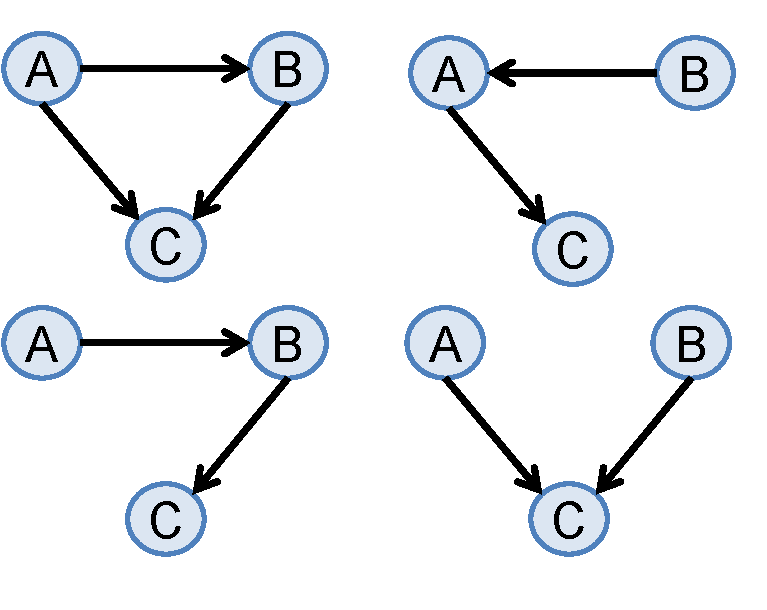
\includegraphics[width=0.4\textwidth]{figures/example-net-structures.pdf}
% \end{center}
% \caption{Examples of possible network structures}\label{example-net-structures}
% \end{figure}


\section{Experiments and Results}
We evaluate our relation entailment graphs on the database query task, as described in section~\ref{database-query-task}. The queries we chose to evaluate over are listed in table~\ref{benchmark-queries}. The first five queries we chose originally, and the final ten we chose to exercise the relation entailment graph we obtained through Bayesian network structure learning. Without the final 10 queries, structure learning performs the same as the baseline, since there are no expansions as shown in table~\ref{results}.

\begin{table}[h]
  \caption{Benchmark queries for database query task. The first five queries we chose originally, and the final ten we chose to exercise our structure learning graph. }\label{benchmark-queries} 
  \begin{center}
    \sffamily 
    \begin{tabular}{l}
      \toprule
      \textrm{Query}\\
      \midrule
      has-written(type: Person, type: Book)\\
      play(Tom Hanks, ?)\\
      conquer(?, Egypt)\\
      killed(?, Voldemort)\\
      grown-in(coffee, type: Country)\\
      \midrule
      be-one-of(coffee, type:Country)\\
      work-on(type:Person, type:Book)\\
      be-solidly-establish in(coffee, type:Country)\\
      believe-in(type:Person, type:Book)\\
      play-major-economic-role-in(coffee, type:Country)\\
      be-come-in(type:Person, type:Book)\\
      discuss-character-of(Tom Hanks, ?)\\
      be-originally-find-in(coffee, type:Country)\\
      tell(Tom Hanks, ?)\\
      endorse(Tom Hanks, ?)\\
      \bottomrule
    \end{tabular}
  \end{center}
\end{table}


Our baseline is a system that does no query expansion, only searching the database for an exact string match of the relation phrase. We compare this to systems that expand queries based on the entailment graphs from 1) all of WordNet, 2) WordNet with logistic regression, and 3) Bayesian network structure learning.

We manually labeled the results from out WordNet-based system without logistic regression, and trained the logistic regression model on the labeled data using 10-fold cross validation.

We used the Bayes Net Toolbox for Matlab \cite{murphy2001bayes} to perform Bayesian network structure learning. The input to the structure learning was a counts matrix, with relation phrases for rows and entity-entity pairs for columns. However, we were constrained by high memory usage when running structure learning on graphs with more than 150 relation phrases. As a result, for some queries, we had to randomly sample 150 relation phrases. The search was done using 100 samples of MCMC, with a burn-in of 10 samples. We used tabular CPDs, boolean variables representing whether the relation holds, and searched according to equation~\ref{eqn:dpsm} with a uniform prior ($N^\prime_{ijk} = 1$). We smoothed the counts by adding $\epsilon = 0.1$ to the counts matrix. 


% Structure learning had no effect on the results, because none of the entailments learned through structure learning applied to the five queries listed in table~\ref{benchmark-queries}.

% To see the results of structure learning, we also tried a set of 10 benchmark queries that had entries in the entailment graph generated from structure learning. The queries are listed in table~\ref{structure-queries}, and our results are shown in table~\ref{structure-results}.

Our results are summarized in table~\ref{combined-results}. These results show that using entailments from WordNet improved recall substantially. We were surprised that using WordNet entailments did not decrease precision more than it did, but that likely stems from our choice of queries. For example, while not many facts in the database specifically say a person ``has written'' a book, many facts say a person ``writes'' a book. Since we consider those to be correct answers, those results push precision up. Adding the logistic regression classifier presented us with a precision/yield tradeoff but does result in a higher precision than the baseline with over 6x more results.

This set of results shows that our structure learning will increase the number of results returned, but at a high cost to precision. Our results also show that for the more specific queries presented in the final 10 entries of table~\ref{benchmark-queries}, almost all of the extra results given by WordNet entailments are bad (see table~\ref{structure-results}). The classifier partially recovered the loss in precision.


\begin{table}[h]
  \caption{Results on database query task for the first five queries in table~\ref{benchmark-queries} (initial benchmark queries).}\label{results}
  \begin{center}
    \begin{tabular}{l l l}
      \toprule
      System & \# results returned & Precision\\
      \midrule
      Baseline & 115 & 83.48\%\\
      Structure learning & 115 & 83.48\%\\
      WordNet & 1105 & 86.85\% \\
      WordNet + logistic regression & 1035 & 91.50\%\\
      \bottomrule
    \end{tabular}
  \end{center}
\end{table}



\begin{table}[h]
  \caption{Results on database query task for the final ten queries in table~\ref{benchmark-queries} (more specific queries to exercise structure learning).}\label{structure-results}
  \begin{center}
    \begin{tabular}{l l l}
      \toprule
      System & \# results returned & Precision\\
      \midrule
      Baseline & 55 & 98.18\%\\
      Structure learning & 73 & 76.71\%\\
      WordNet & 108 & 56.48\% \\
      WordNet + logistic regression & 58 & 91.38\%\\
      \bottomrule
    \end{tabular}
  \end{center}
\end{table}


\begin{table}[h]
  \caption{Results on database query task for all queries in table~\ref{benchmark-queries}.}\label{combined-results}
  \begin{center}
    \begin{tabular}{l l l}
      \toprule
      System & \# results returned & Precision\\
      \midrule
      Baseline & 165 & 87.88\%\\
      Structure learning & 183 & 80.33\%\\
      WordNet & 1188 & 84.09\% \\
      WordNet + logistic regression & 1097 & 91.43\%\\
      \bottomrule
    \end{tabular}
  \end{center}
\end{table}

\section{Discussion and Conclusion}

In this project we tried two approaches to learning relation entailment graphs: Bayesian network structured learning and using logistic regression to intelligently map entailments to WordNet. Using these methods to expand relation queries, we find that Bayesian network structure learning reduces precision, because we were not able to find a way to bias the directionality of edges in a way appropriate for the problem; however, using WordNet with logistic regression increased the number of results returned by over 6x while increasing precision from 87.88\% to 91.43\% for the 15 example queries.

Our results suggest that the choice of benchmark queries can make a big difference in the results. However, we noticed that using WordNet with a classifier does seem to increase yield at an acceptable level of precision. Although it's hard to say what queries should be used in our experiment, the first five queries in table~\ref{benchmark-queries} are arguably more common than the final 10.

Berant, et al. use both symmetric and asymmetric metrics to represent the relation entailment problem in order to capture edge directionality \cite{Berant:2012:LER:2122944.2122947}. They use an asymmetric \textit{Cover} measure, which assumes that if one predicate entails another, relatively many of the features of the entailing predicate should be covered by that of the entailed predicate. This could be adapted as a term for structure learning to bias the scores based on if instances (entity-entity pairs) of one relation are covered by another, or this could be performed as a postprocessing stage on the learned relation entailment graph. Another possiblity could be to learn a supervised classifier over edge direction using features including instance cover as well as other metrics like those in~\cite{Berant:2012:LER:2122944.2122947}.

An alternative way to model this problem of relation entailment could be based on using the relational Markov network framework of~\cite{Taskar:2002:DPM:2073876.2073934} to predict links as in~\cite{TaskarWAK03}. In~\cite{TaskarWAK03} relational schemas are defined with object types and attributes. They use the domain of university webpage, where both pages and links are objects, and attributes can be information such as from a bag of words. A RMN is defined to provide cliques and potentials between attributes of related entities using templates, such as between class labels of linked pages. The parameters are learned from data over a single relational instantiation using belief propagation. We could model the entities and relations that we are dealing with in a similar way. Instead of pages we would have entities, instead of links we would have relations or relation strings, and potentially we could have entity types, either from Freebase or latent for labels. The cliques could group together entities appearing in the same sentence or document. Then the relation extraction problem would be to learn more links given some observed links, and the relation entailment problem could be approached by extracting the probabilities of one kind of link given another and forming a corresponding relation entailment graph that agrees.


\bibliographystyle{abbrv}
\bibliography{bib}

\end{document}
